\section{Carrot Stew}
\cofeAm{1}{1}{180}{0}{0}
\begin{centering}

Serves

\end{centering}

\begin{table}[H]
  \centering
    
  \begin{tabular*}{1\textwidth}{rlrl}
      % &  & &  \\
    17.5\,oz & carrots  & 13.2\,oz & minced meat (beef) \\
	7\,oz & potatoes (optional) & & garlic flavoured salt \\
	2\,tbs & butter & & onion flavoured salt\\
	2 cups/16.9\,fl oz & (vegetable) stock & & wocester sauce \\
	2-3 sticks & leek & 1 bunch & parsley \\
	& salt, pepper &  & \\
  \end{tabular*}
\end{table}

%Zubereitung:
\begin{Notes}
\item Clean carrots/potatoes and slice into sticks. In 1\,tbs butter saut\'{e} vegetables, then add vegetable stock. Cover and let boil lightly for about 10\,min. Cut leek into rings, wash and add to the carrots. Season with salt and pepper.
\item Season minced meat with pepper, salt and garlic and onion flavoured salt. Let 1\,tbs butter melt in a pan and saut\'{e} meat. Season to taste with worcester sauce and add to the vegetables.
\item Chop parsley and serve carrot stew with parsley on top.
\end{Notes}
\vfill
\begin{figure}[H]
  \centering
  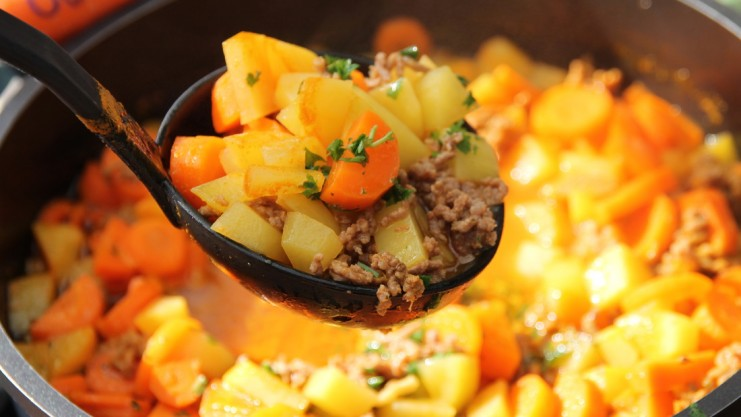
\includegraphics[width=0.65\textwidth]{moeheneintopf.jpg}
\end{figure}
\newpage

\section*{M\"{o}hreneintopf}

\begin{centering}

F\"{u}r

\end{centering}

\begin{table}[H]
  \centering
    
  \begin{tabular*}{1\textwidth}{rlrl}
      % &  & &  \\
    500\,g & M\"{o}hren  & 375\,g & (Rinder-)Hackfleisch \\
	200\,g & Kartoffeln (optional) & & Knoblauchsalz \\
	2\,EL & Butter & & Zwiebelsalz \\
	\nicefrac{1}{2}\,l & Br\"{u}he &  & Wocestersauce \\
	2-3 Stangen & Lauch & 1 Bd.& Petersilie \\
	& Salz, Pfeffer &  & \\
  \end{tabular*}
\end{table}

%Zubereitung:
\begin{Notes}
\item Die M\"{o}hren/Kartoffeln waschen, putzen und in Stifte schneiden, in 1\,EL Butter kurz and\"{u}nsten und mit der Br\"{u}he auff\"{u}llen. Zugedeckt etwa 10\,min k\"{o}cheln lassen. Den Lauch in Ringe schneiden, waschen und hinzuf\"{u}gen, mit Salz und Pfeffer w\"{u}rzen.
\item Rinderhack mit Pfeffer, Salz und, nach Geschmack, mit Knoblauch- und Zwiebelsalz w\"{u}rzen und in einer Pfanne mit 1\,EL Butter anbraten. Mit Worcestersauce w\"{u}rzen und zu dem Gem\"{u}se geben.
\item Petersilie hacken und Eintopf mit Petersilie bestreut servieren.
\end{Notes}
\vfill
\begin{figure}[H]
  \centering
  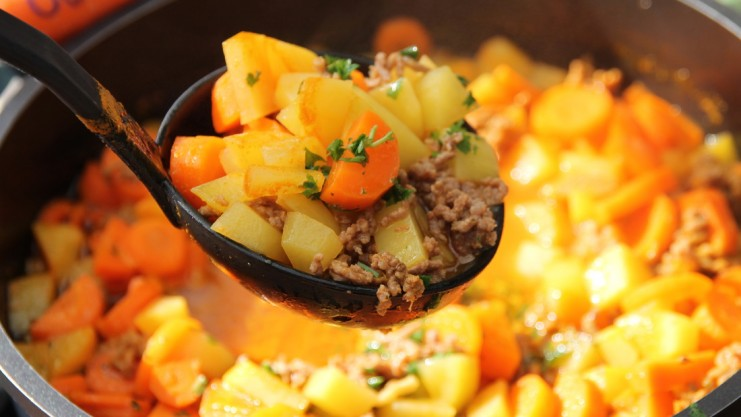
\includegraphics[width=0.65\textwidth]{moeheneintopf.jpg}
\end{figure}
\newpage
